% Options for packages loaded elsewhere
\PassOptionsToPackage{unicode}{hyperref}
\PassOptionsToPackage{hyphens}{url}
\PassOptionsToPackage{dvipsnames,svgnames,x11names}{xcolor}
%
\documentclass[
  a4paper,
  DIV=11,
  numbers=noendperiod]{scrartcl}

\usepackage{amsmath,amssymb}
\usepackage{iftex}
\ifPDFTeX
  \usepackage[T1]{fontenc}
  \usepackage[utf8]{inputenc}
  \usepackage{textcomp} % provide euro and other symbols
\else % if luatex or xetex
  \usepackage{unicode-math}
  \defaultfontfeatures{Scale=MatchLowercase}
  \defaultfontfeatures[\rmfamily]{Ligatures=TeX,Scale=1}
\fi
\usepackage{lmodern}
\ifPDFTeX\else  
    % xetex/luatex font selection
\fi
% Use upquote if available, for straight quotes in verbatim environments
\IfFileExists{upquote.sty}{\usepackage{upquote}}{}
\IfFileExists{microtype.sty}{% use microtype if available
  \usepackage[]{microtype}
  \UseMicrotypeSet[protrusion]{basicmath} % disable protrusion for tt fonts
}{}
\makeatletter
\@ifundefined{KOMAClassName}{% if non-KOMA class
  \IfFileExists{parskip.sty}{%
    \usepackage{parskip}
  }{% else
    \setlength{\parindent}{0pt}
    \setlength{\parskip}{6pt plus 2pt minus 1pt}}
}{% if KOMA class
  \KOMAoptions{parskip=half}}
\makeatother
\usepackage{xcolor}
\usepackage[inner=2.5cm,outer=2.5cm,top=3cm,bottom=4cm,headsep=22pt,headheight=11pt,footskip=33pt,ignorehead,ignorefoot,heightrounded]{geometry}
\setlength{\emergencystretch}{3em} % prevent overfull lines
\setcounter{secnumdepth}{5}
% Make \paragraph and \subparagraph free-standing
\makeatletter
\ifx\paragraph\undefined\else
  \let\oldparagraph\paragraph
  \renewcommand{\paragraph}{
    \@ifstar
      \xxxParagraphStar
      \xxxParagraphNoStar
  }
  \newcommand{\xxxParagraphStar}[1]{\oldparagraph*{#1}\mbox{}}
  \newcommand{\xxxParagraphNoStar}[1]{\oldparagraph{#1}\mbox{}}
\fi
\ifx\subparagraph\undefined\else
  \let\oldsubparagraph\subparagraph
  \renewcommand{\subparagraph}{
    \@ifstar
      \xxxSubParagraphStar
      \xxxSubParagraphNoStar
  }
  \newcommand{\xxxSubParagraphStar}[1]{\oldsubparagraph*{#1}\mbox{}}
  \newcommand{\xxxSubParagraphNoStar}[1]{\oldsubparagraph{#1}\mbox{}}
\fi
\makeatother


\providecommand{\tightlist}{%
  \setlength{\itemsep}{0pt}\setlength{\parskip}{0pt}}\usepackage{longtable,booktabs,array}
\usepackage{calc} % for calculating minipage widths
% Correct order of tables after \paragraph or \subparagraph
\usepackage{etoolbox}
\makeatletter
\patchcmd\longtable{\par}{\if@noskipsec\mbox{}\fi\par}{}{}
\makeatother
% Allow footnotes in longtable head/foot
\IfFileExists{footnotehyper.sty}{\usepackage{footnotehyper}}{\usepackage{footnote}}
\makesavenoteenv{longtable}
\usepackage{graphicx}
\makeatletter
\def\maxwidth{\ifdim\Gin@nat@width>\linewidth\linewidth\else\Gin@nat@width\fi}
\def\maxheight{\ifdim\Gin@nat@height>\textheight\textheight\else\Gin@nat@height\fi}
\makeatother
% Scale images if necessary, so that they will not overflow the page
% margins by default, and it is still possible to overwrite the defaults
% using explicit options in \includegraphics[width, height, ...]{}
\setkeys{Gin}{width=\maxwidth,height=\maxheight,keepaspectratio}
% Set default figure placement to htbp
\makeatletter
\def\fps@figure{htbp}
\makeatother
% definitions for citeproc citations
\NewDocumentCommand\citeproctext{}{}
\NewDocumentCommand\citeproc{mm}{%
  \begingroup\def\citeproctext{#2}\cite{#1}\endgroup}
\makeatletter
 % allow citations to break across lines
 \let\@cite@ofmt\@firstofone
 % avoid brackets around text for \cite:
 \def\@biblabel#1{}
 \def\@cite#1#2{{#1\if@tempswa , #2\fi}}
\makeatother
\newlength{\cslhangindent}
\setlength{\cslhangindent}{1.5em}
\newlength{\csllabelwidth}
\setlength{\csllabelwidth}{3em}
\newenvironment{CSLReferences}[2] % #1 hanging-indent, #2 entry-spacing
 {\begin{list}{}{%
  \setlength{\itemindent}{0pt}
  \setlength{\leftmargin}{0pt}
  \setlength{\parsep}{0pt}
  % turn on hanging indent if param 1 is 1
  \ifodd #1
   \setlength{\leftmargin}{\cslhangindent}
   \setlength{\itemindent}{-1\cslhangindent}
  \fi
  % set entry spacing
  \setlength{\itemsep}{#2\baselineskip}}}
 {\end{list}}
\usepackage{calc}
\newcommand{\CSLBlock}[1]{\hfill\break\parbox[t]{\linewidth}{\strut\ignorespaces#1\strut}}
\newcommand{\CSLLeftMargin}[1]{\parbox[t]{\csllabelwidth}{\strut#1\strut}}
\newcommand{\CSLRightInline}[1]{\parbox[t]{\linewidth - \csllabelwidth}{\strut#1\strut}}
\newcommand{\CSLIndent}[1]{\hspace{\cslhangindent}#1}

\KOMAoption{captions}{tableheading}
\makeatletter
\@ifpackageloaded{tcolorbox}{}{\usepackage[skins,breakable]{tcolorbox}}
\@ifpackageloaded{fontawesome5}{}{\usepackage{fontawesome5}}
\definecolor{quarto-callout-color}{HTML}{909090}
\definecolor{quarto-callout-note-color}{HTML}{0758E5}
\definecolor{quarto-callout-important-color}{HTML}{CC1914}
\definecolor{quarto-callout-warning-color}{HTML}{EB9113}
\definecolor{quarto-callout-tip-color}{HTML}{00A047}
\definecolor{quarto-callout-caution-color}{HTML}{FC5300}
\definecolor{quarto-callout-color-frame}{HTML}{acacac}
\definecolor{quarto-callout-note-color-frame}{HTML}{4582ec}
\definecolor{quarto-callout-important-color-frame}{HTML}{d9534f}
\definecolor{quarto-callout-warning-color-frame}{HTML}{f0ad4e}
\definecolor{quarto-callout-tip-color-frame}{HTML}{02b875}
\definecolor{quarto-callout-caution-color-frame}{HTML}{fd7e14}
\makeatother
\makeatletter
\@ifpackageloaded{caption}{}{\usepackage{caption}}
\AtBeginDocument{%
\ifdefined\contentsname
  \renewcommand*\contentsname{Table of contents}
\else
  \newcommand\contentsname{Table of contents}
\fi
\ifdefined\listfigurename
  \renewcommand*\listfigurename{List of Figures}
\else
  \newcommand\listfigurename{List of Figures}
\fi
\ifdefined\listtablename
  \renewcommand*\listtablename{List of Tables}
\else
  \newcommand\listtablename{List of Tables}
\fi
\ifdefined\figurename
  \renewcommand*\figurename{Figure}
\else
  \newcommand\figurename{Figure}
\fi
\ifdefined\tablename
  \renewcommand*\tablename{Table}
\else
  \newcommand\tablename{Table}
\fi
}
\@ifpackageloaded{float}{}{\usepackage{float}}
\floatstyle{ruled}
\@ifundefined{c@chapter}{\newfloat{codelisting}{h}{lop}}{\newfloat{codelisting}{h}{lop}[chapter]}
\floatname{codelisting}{Listing}
\newcommand*\listoflistings{\listof{codelisting}{List of Listings}}
\makeatother
\makeatletter
\makeatother
\makeatletter
\@ifpackageloaded{caption}{}{\usepackage{caption}}
\@ifpackageloaded{subcaption}{}{\usepackage{subcaption}}
\makeatother

\ifLuaTeX
  \usepackage{selnolig}  % disable illegal ligatures
\fi
\usepackage{bookmark}

\IfFileExists{xurl.sty}{\usepackage{xurl}}{} % add URL line breaks if available
\urlstyle{same} % disable monospaced font for URLs
\hypersetup{
  pdftitle={GovSteamEU},
  pdfauthor={Martin Franke, Saikrishna Vallabhaneni, Nils Wiese},
  colorlinks=true,
  linkcolor={blue},
  filecolor={Maroon},
  citecolor={Blue},
  urlcolor={Blue},
  pdfcreator={LaTeX via pandoc}}


\title{GovSteamEU}
\author{Martin Franke, Saikrishna Vallabhaneni, Nils Wiese}
\date{}

\begin{document}
\maketitle

\renewcommand*\contentsname{Table of contents}
{
\hypersetup{linkcolor=}
\setcounter{tocdepth}{3}
\tableofcontents
}
\listoffigures
\listoftables

\section{Context}\label{context}

The traditional operation of electrical power systems depends on the
performance of the synchronous generators of thermal plants, typically
driven by various types of turbines such as steam, gas, or hydro
turbines. Steam turbines are commonly found in coal, oil, and nuclear
power plants. The process begins with the generation of high-pressure
high-temperature steam in a boiler. A governor regulates the mechanical
power (\(P_m\)) delivered from the turbine to the electrical generator.
Modern governors with electro-hydraulic control, like the GovSteamEU,
evolved from governors with mechanical-hydraulic control.

GovSteamEU is documented in {[}1{]}. Many aspects of modeling steam
governors with electro-hydraulic control are already explained in a 1973
IEEE report {[}2{]}.

\section{Model use, assumptions, validity domain and
limitations}\label{model-use-assumptions-validity-domain-and-limitations}

The model is a positive-sequence RMS model, hence it assumes symmetrical
operating conditions and neglects high-frequency dynamics. This type of
model is often used in large-scale stability studies, for which it
reflects the relevant phenomena. It is not a detailed physical model of
the unit. Also for some stability phenomena (e.g.~resonance stability)
this model is not sufficient and EMT models or other approaches may be
necessary .

The model operates only under the assumption that resistive and
mechanical losses are negligible, and in steady state condition
\(P_\mathrm{e} = P_\mathrm{m}\). This assumes that mechanical losses do
not have any major effect on dynamic stability {[}1{]}.

\section{Model schema}\label{model-schema}

\begin{figure}

\centering{

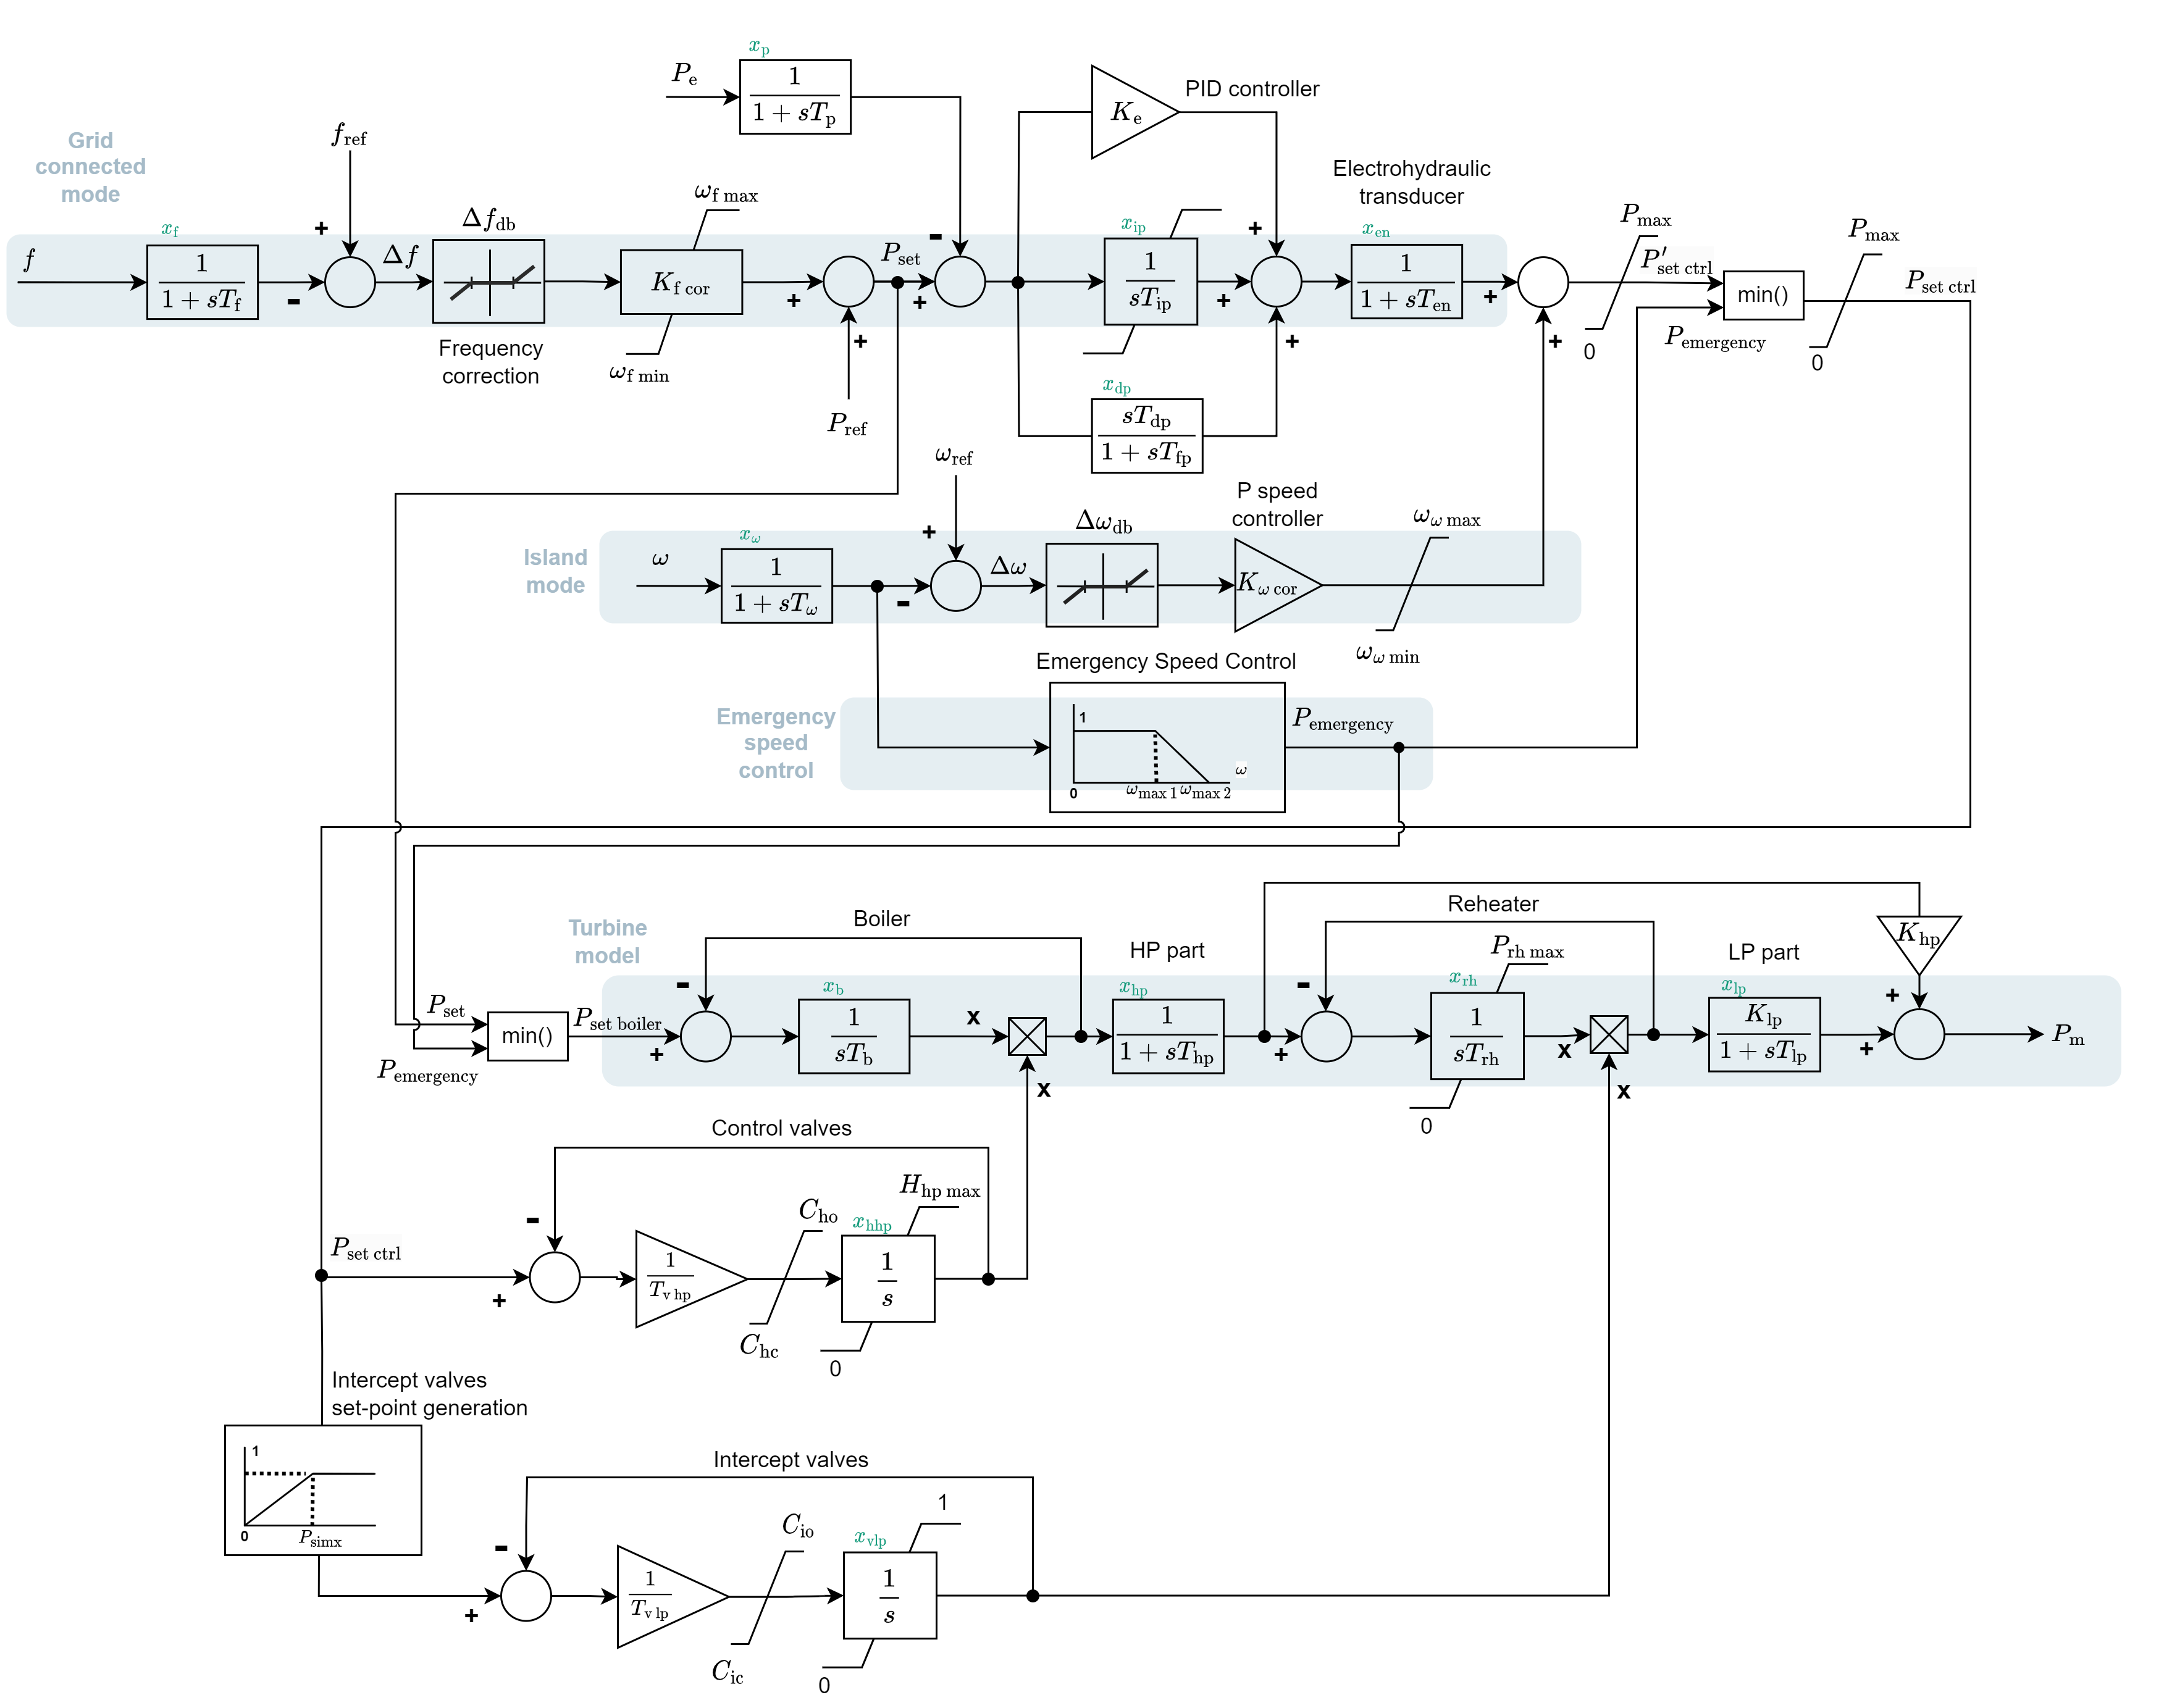
\includegraphics{./drawings/GovSteamEU.drawio.png}

}

\caption{\label{fig-control_diagram}Model schema, based on {[}1{]} and
{[}3{]}}

\end{figure}%

\begin{figure}

\centering{

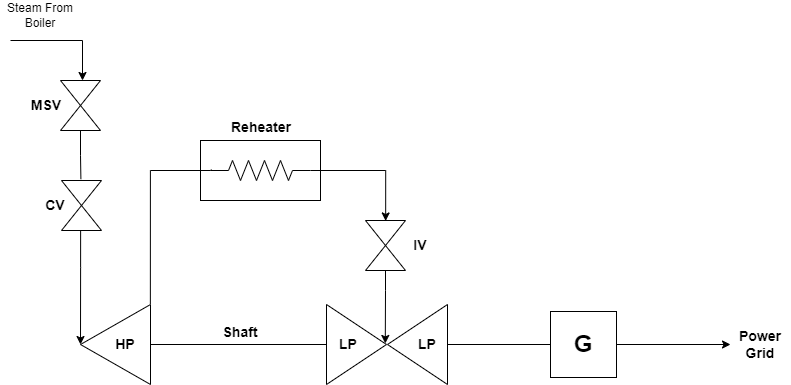
\includegraphics{./drawings/SteamTurbineConfig.drawio.png}

}

\caption{\label{fig-Steam_turbine_configuration}Steam turbine with high
pressure (HP) and low pressure (LP) part}

\end{figure}%

\section{Model description}\label{model-description}

\subsection{Turbine model}\label{turbine-model}

The turbine model is the mechanical part of the model with boiler, high
pressure (HP) turbine and low pressure (LP) turbine {[}4{]}. Its output
is the mechanical power \(P_\mathrm{m}\). A schematic representation of
a steam turbine with HP and LP part is shown in
Figure~\ref{fig-Steam_turbine_configuration}. The HP stage's
single-triangle symbol and the LP stage's double-triangle symbol
represent the fact that in the HP stage steam expands in only one
direction whereas in the LP stage it expands in two directions {[}5{]}.

\subsubsection{Boiler}\label{boiler}

The boiler is responsible for converting water into high-pressure,
high-temperature steam. In normal operation \(P_\mathrm{set}\) is used
as the boiler set-point \(P_\mathrm{set\,boiler}\), i.e.~the heat
supplied to the boiler. In over speed situation, the emergency speed
control signal is used instead, see Section~\ref{sec-emergency}.

The boiler output, i.e.~the amount of steam supplied from the boiler to
the turbine, is manipulated by the control valves {[}4{]}.

\subsubsection{High-Pressure (HP) and low pressure (LP) turbine
stages}\label{high-pressure-hp-and-low-pressure-lp-turbine-stages}

The HP and LP stages are modeled by a first order elements and gains
\(T_\mathrm{hp}\), \(K_\mathrm{hp}\) and \(T_\mathrm{lp}\),
\(K_\mathrm{lp}\).

Steam power from the boiler enters the HP stage and is partly converted
into mechanical power. The steam output from the HP stage then enters
the reheater. Because the HP stage's dynamic response is relevant here,
the output of the \(T_\mathrm{hp}\) lag element is used as input, but
without the gain \(K_\mathrm{hp}\).

Before entering the LP stage, the output steam from the HP stage must be
reheated to prevent any water droplets from entering and to increase
efficiency. The reheater is also modeled by a first order element with
time constant \(T_\mathrm{rh}\).

From there the reheated steam passes the intercept valve and enters the
LP stage. Here, the first order element directly contains the gain
\(K_\mathrm{lp}\), because only the generated power is of interest (the
dynamic behaviour of the steam flow without gain is not necessary
because there is no other following turbine stage) {[}4{]}.

The mechanical power output \(P_\mathrm{m}\) is the sum of the parts
generated by the HP and LP turbine stages. To accurately represent this
distribution, the gains for the HP and LP turbine stages must satisfy
the following condition:

\[K_\mathrm{hp} + K_\mathrm{lp}  = 1\]

\subsection{Control paths}\label{control-paths}

The governor controller is responsible for regulating the steam flow to
maintain the desired turbine speed or power output. It consists of two
primary control paths {[}4{]}, island and grid connected mode. They
output the setpoint of the control valve's position.

\subsubsection{\texorpdfstring{Island mode
(\(\omega\)-part)}{Island mode (\textbackslash omega-part)}}\label{island-mode-omega-part}

In island mode, the input is the turbine's rotational speed \(\omega\).
It operates without connection to any external power grid, with the
primary goal of maintaining a constant turbine speed. To achieve this,
the measured turbine speed \(\omega\) is subtracted from the reference
speed \(\omega_\mathrm{ref}\) to obtain the error signal
\(\Delta\omega\). After passing the dead-band
\(\Delta \omega_\mathrm{db}\), it is used as input for the proportional
\(K_\mathrm{\omega\,cor}\) {[}4{]} {[}6{]}.

\subsubsection{\texorpdfstring{Grid connected mode
(\(f\)-part)}{Grid connected mode (f-part)}}\label{grid-connected-mode-f-part}

In grid connected mode, the input is the measured electrical frequency
\(f\). The plant is linked to an upstream grid and contributes to
overall grid stability. Here, frequency control is achieved through
collective behavior; individual output adjustments are made via droop
regulation.

This is implemented via a proportional gain \(K_\mathrm{f\,cor}\) with
dead-band \(\Delta f_\mathrm{db}\) contributing to the power set-point
\(P_\mathrm{set}\). The measured power \(P_\mathrm{e}\) is then
subtracted to obtain the error signal \(\Delta f\) of the PID controller
{[}4{]} {[}6{]}.

\subsubsection{Emergency speed control and intercept valve
(IV)}\label{sec-emergency}

\textbf{Emergency speed control}

In case of loss of loads, the turbine speed instantly begins to
increase. Ideally, the governor is able to handle such fluctuations and
reduces the control valve set-point fast enough. If not, an emergency
speed control is activated to reduce the active power output of the
turbine fast.

The \emph{Emergency Speed Control} block in
Figure~\ref{fig-control_diagram} outputs 1 if
\(\omega < \omega_\mathrm{max\,1}\) and 0 if
\(\omega > \omega_\mathrm{max\,2}\). In-between it interpolates between
1 and 0. This output is supposed to be below 1 or equal to 0 if
\(\omega\) reaches dangerous levels (dangerous for mechanical stability
of the turbine). It is then passed to the two different low value select
blocks (min()).

This has the effect of reducing the control valve and boiler set-points
(\(P_\mathrm{set\,ctrl}\), \(P_\mathrm{set\,boiler}\)) fast,
independently of what the controllers and the power set-point
\(P_\mathrm{set}\) do.

This fast reduction of \(P_\mathrm{set\,ctrl}\) also affects the
intercept valve model, see below.

\textbf{Intercept valve (IV)}

Intercept valves remain fully open (set-point and position = 1) for
regular speed/load adjustments {[}4{]}. In overspeed situations, the
intercept valve shall close quickly and then reopen once normal
conditions are restored.

In this model, the intercept valve set-point is generated by the
\emph{intercept valves set-point generation} block. The input is the
control valves input signal.

If the control valve set-point \(P_\mathrm{set\,ctrl}\) is above
\(P_\mathrm{simx}\), the output is 1. If \(P_\mathrm{set\,ctrl}\) drops
below, the output is reduced linearly until it reaches 0. In other
implementations, a step to 0 is used instead of linear reduction as
shown in the Figure~\ref{fig-control_diagram} from {[}1{]}.

In combination with the emergency speed control block, this leads to a
fast reduction of the intercept valve set-point in case of over speed
and hence interrupting the steam flow into the LP turbine and quickly
reducing \(P_\mathrm{m}\).

\section{Parameters:}\label{parameters}

The parameters are based on {[}1{]} and {[}3{]}.

Per-unit parameters are on base of \(P_\mathrm{base}\), which is
normally the capability of the turbine in MW.

\begin{longtable}[]{@{}
  >{\raggedright\arraybackslash}p{(\columnwidth - 12\tabcolsep) * \real{0.0600}}
  >{\raggedright\arraybackslash}p{(\columnwidth - 12\tabcolsep) * \real{0.0600}}
  >{\raggedright\arraybackslash}p{(\columnwidth - 12\tabcolsep) * \real{0.0500}}
  >{\raggedright\arraybackslash}p{(\columnwidth - 12\tabcolsep) * \real{0.2500}}
  >{\raggedright\arraybackslash}p{(\columnwidth - 12\tabcolsep) * \real{0.1200}}
  >{\raggedright\arraybackslash}p{(\columnwidth - 12\tabcolsep) * \real{0.3800}}
  >{\raggedright\arraybackslash}p{(\columnwidth - 12\tabcolsep) * \real{0.0700}}@{}}
\caption{Parameters}\label{tbl-parameters}\tabularnewline
\toprule\noalign{}
\begin{minipage}[b]{\linewidth}\raggedright
name
\end{minipage} & \begin{minipage}[b]{\linewidth}\raggedright
type
\end{minipage} & \begin{minipage}[b]{\linewidth}\raggedright
unit
\end{minipage} & \begin{minipage}[b]{\linewidth}\raggedright
modelica name
\end{minipage} & \begin{minipage}[b]{\linewidth}\raggedright
IEC name
\end{minipage} & \begin{minipage}[b]{\linewidth}\raggedright
description
\end{minipage} & \begin{minipage}[b]{\linewidth}\raggedright
typical value
\end{minipage} \\
\midrule\noalign{}
\endfirsthead
\toprule\noalign{}
\begin{minipage}[b]{\linewidth}\raggedright
name
\end{minipage} & \begin{minipage}[b]{\linewidth}\raggedright
type
\end{minipage} & \begin{minipage}[b]{\linewidth}\raggedright
unit
\end{minipage} & \begin{minipage}[b]{\linewidth}\raggedright
modelica name
\end{minipage} & \begin{minipage}[b]{\linewidth}\raggedright
IEC name
\end{minipage} & \begin{minipage}[b]{\linewidth}\raggedright
description
\end{minipage} & \begin{minipage}[b]{\linewidth}\raggedright
typical value
\end{minipage} \\
\midrule\noalign{}
\endhead
\bottomrule\noalign{}
\endlastfoot
\(C_\mathrm{hc}\) & float & pu & CHcPu & chc & Control valves closing
rate limit & -3.3 \\
\(C_\mathrm{ho}\) & float & pu & CHoPu & cho & Control valves opening
rate limit & 0.17 \\
\(C_\mathrm{ic}\) & float & pu & CIcPu & cic & Intercept valves closing
rate limit & -2.2 \\
\(C_\mathrm{io}\) & float & pu & CIoPu & cio & Intercept valves opening
rate limit & 0.123 \\
\(\Delta f_\mathrm{db}\) & float & pu & db1Pu & db1 & Deadband of
frequency droop & 0 \\
\(\Delta\omega_\mathrm{db}\) & float & pu & db2Pu & db2 & Deadband of
the speed governor (island mode) & 0.0004 \\
\(H_\mathrm{hp\,max}\) & float & pu & HHpMaxPu & hhpmax & Maximum
control valve position & 1 \\
\(K_\mathrm{e}\) & float & pu & KE & ke & Proportional gain of the PID
controller & 0.65 \\
\(K_\mathrm{f\,cor}\) & float & pu & KFCor & kfcor & Frequency droop &
20 \\
\(K_\mathrm{hp}\) & float & pu & KHp & khp & Fraction of total turbine
output generated by HP part & 0.277 \\
\(K_\mathrm{lp}\) & float & pu & KLp & klp & Fraction of total turbine
output generated by LP part & 0.723 \\
\(K_{\mathrm{\omega\,cor}}\) & float & pu & KOmegaCor & komegacor & Gain
of the speed governor (island mode) & 20 \\
\(\omega_\mathrm{f\,max}\) & float & pu & OmegaFMaxPu & wfmax & Upper
limit for droop output & 0.05 \\
\(\omega_\mathrm{f\,min}\) & float & pu & OmegaFMinPu & wfmin & Lower
limit for droop output & -0.05 \\
\(\omega_\mathrm{max\,1}\) & float & pu & OmegaMax1Pu & wmax1 &
Emergency speed control lower limit & 1.025 \\
\(\omega_\mathrm{max\,2}\) & float & pu & OmegaMax2Pu & wmax2 &
Emergency speed control upper limit & 1.05 \\
\(\omega_\mathrm{\omega\,max}\) & float & pu & OmegaOmegaMaxPu & wwmax &
Upper limit for the speed governor (island mode) & 0.1 \\
\(\omega_\mathrm{\omega\,min}\) & float & pu & OmegaOmegaMinPu & wwmin &
Lower limit for the speed governor (island mode) & -1 \\
\(P_\mathrm{max}\) & float & pu & PMaxPu & pmax & Maximal active power
of the turbine & 1 \\
\(P_\mathrm{rh\,max}\) & float & pu & PRhMaxPu & prhmax & Maximum low
pressure limit & 1.4 \\
\(P_\mathrm{simx}\) & float & pu & SimxPu & simx & Intercept valves
transfer limit & 0.425 \\
\(T_\mathrm{b}\) & float & s & tB & tb & Boiler time constant & 100 \\
\(T_\mathrm{dp}\) & float & s & tDp & tdp & Derivative time constant of
the power controller & 0 \\
\(T_\mathrm{en}\) & float & s & tEht & ten & Electro hydraulic
transducer & 0.1 \\
\(T_\mathrm{f}\) & float & s & tFt & tf & Frequency transducer time
constant & 0 \\
\(T_\mathrm{fp}\) & float & s & tFp & tfp & Time constant for nunmerical
approximation of PID controller derivative part & 0 \\
\(T_\mathrm{hp}\) & float & s & tHpt & thp & High pressure (HP) time
constant of the turbine & 0.31 \\
\(T_\mathrm{ip}\) & float & s & tIPc & tip & Integral time constant of
PID controller & 2 \\
\(T_\mathrm{lp}\) & float & s & tLpt & tlp & Low pressure (LP) time
constant of the turbine & 0.45 \\
\(T_\mathrm{\omega}\) & float & s & tOmega & tw & Speed transducer time
constant & 0.02 \\
\(T_\mathrm{p}\) & float & s & tPt & tp & Power transducer time constant
& 0.07 \\
\(T_\mathrm{rh}\) & float & s & tRh & trh & Reheater time constant of
the turbine & 8 \\
\(T_\mathrm{v\,hp}\) & float & s & tCv & tvhp & Control valves servo
time constant & 0.1 \\
\(T_\mathrm{v\,lp}\) & float & s & tIv & tvlp & Intercept valves servo
time constant & 0.15 \\
\end{longtable}

\begin{tcolorbox}[enhanced jigsaw, colback=white, bottomrule=.15mm, breakable, title=\textcolor{quarto-callout-note-color}{\faInfo}\hspace{0.5em}{Note}, arc=.35mm, toprule=.15mm, rightrule=.15mm, coltitle=black, bottomtitle=1mm, leftrule=.75mm, colframe=quarto-callout-note-color-frame, left=2mm, toptitle=1mm, titlerule=0mm, opacitybacktitle=0.6, colbacktitle=quarto-callout-note-color!10!white, opacityback=0]

As stated in {[}1{]}, to represent a turbine without a reheater, set
\(T_\mathrm{rh} =\) 0 s and \(T_\mathrm{lp} \approx\) 0.5 s .

\end{tcolorbox}

\section{Variables}\label{variables}

\subsection{Inputs}\label{inputs}

\begin{longtable}[]{@{}
  >{\raggedright\arraybackslash}p{(\columnwidth - 10\tabcolsep) * \real{0.1951}}
  >{\raggedright\arraybackslash}p{(\columnwidth - 10\tabcolsep) * \real{0.0610}}
  >{\raggedright\arraybackslash}p{(\columnwidth - 10\tabcolsep) * \real{0.0488}}
  >{\raggedright\arraybackslash}p{(\columnwidth - 10\tabcolsep) * \real{0.1585}}
  >{\raggedright\arraybackslash}p{(\columnwidth - 10\tabcolsep) * \real{0.0976}}
  >{\raggedright\arraybackslash}p{(\columnwidth - 10\tabcolsep) * \real{0.4390}}@{}}
\caption{Inputs}\label{tbl-inputs}\tabularnewline
\toprule\noalign{}
\begin{minipage}[b]{\linewidth}\raggedright
name
\end{minipage} & \begin{minipage}[b]{\linewidth}\raggedright
type
\end{minipage} & \begin{minipage}[b]{\linewidth}\raggedright
unit
\end{minipage} & \begin{minipage}[b]{\linewidth}\raggedright
modelica name
\end{minipage} & \begin{minipage}[b]{\linewidth}\raggedright
IEC name
\end{minipage} & \begin{minipage}[b]{\linewidth}\raggedright
description
\end{minipage} \\
\midrule\noalign{}
\endfirsthead
\toprule\noalign{}
\begin{minipage}[b]{\linewidth}\raggedright
name
\end{minipage} & \begin{minipage}[b]{\linewidth}\raggedright
type
\end{minipage} & \begin{minipage}[b]{\linewidth}\raggedright
unit
\end{minipage} & \begin{minipage}[b]{\linewidth}\raggedright
modelica name
\end{minipage} & \begin{minipage}[b]{\linewidth}\raggedright
IEC name
\end{minipage} & \begin{minipage}[b]{\linewidth}\raggedright
description
\end{minipage} \\
\midrule\noalign{}
\endhead
\bottomrule\noalign{}
\endlastfoot
\(\omega\) & float & pu & omegaPu & \(\omega\) & Rotor speed \\
f & float & pu & f & f & Local (nodal) frequency \\
\(P_\mathrm{e}\) & float & pu & PGenPu & pe & Measured electrical power
generation \\
\(P_\mathrm{ref}\) & float & pu & PRefPu & Pref & load setpoint \\
\end{longtable}

\subsection{Outputs}\label{outputs}

\begin{longtable}[]{@{}
  >{\raggedright\arraybackslash}p{(\columnwidth - 10\tabcolsep) * \real{0.2333}}
  >{\raggedright\arraybackslash}p{(\columnwidth - 10\tabcolsep) * \real{0.0833}}
  >{\raggedright\arraybackslash}p{(\columnwidth - 10\tabcolsep) * \real{0.0667}}
  >{\raggedright\arraybackslash}p{(\columnwidth - 10\tabcolsep) * \real{0.2167}}
  >{\raggedright\arraybackslash}p{(\columnwidth - 10\tabcolsep) * \real{0.1333}}
  >{\raggedright\arraybackslash}p{(\columnwidth - 10\tabcolsep) * \real{0.2667}}@{}}
\caption{Outputs}\label{tbl-outputs}\tabularnewline
\toprule\noalign{}
\begin{minipage}[b]{\linewidth}\raggedright
name
\end{minipage} & \begin{minipage}[b]{\linewidth}\raggedright
type
\end{minipage} & \begin{minipage}[b]{\linewidth}\raggedright
unit
\end{minipage} & \begin{minipage}[b]{\linewidth}\raggedright
modelica name
\end{minipage} & \begin{minipage}[b]{\linewidth}\raggedright
IEC name
\end{minipage} & \begin{minipage}[b]{\linewidth}\raggedright
description
\end{minipage} \\
\midrule\noalign{}
\endfirsthead
\toprule\noalign{}
\begin{minipage}[b]{\linewidth}\raggedright
name
\end{minipage} & \begin{minipage}[b]{\linewidth}\raggedright
type
\end{minipage} & \begin{minipage}[b]{\linewidth}\raggedright
unit
\end{minipage} & \begin{minipage}[b]{\linewidth}\raggedright
modelica name
\end{minipage} & \begin{minipage}[b]{\linewidth}\raggedright
IEC name
\end{minipage} & \begin{minipage}[b]{\linewidth}\raggedright
description
\end{minipage} \\
\midrule\noalign{}
\endhead
\bottomrule\noalign{}
\endlastfoot
\(P_\mathrm{m}\) & float & pu & PmPu & Pm & Mechanical power \\
\end{longtable}

\section{Equations \& algorithm ~}\label{equations-algorithm}

--

\section{Initial equations / boundary conditions
(optional)}\label{initial-equations-boundary-conditions-optional}

The initial values for the system's states are calculated from the
initial mechanical power \(P_\mathrm{m\,0}\), frequency \(f_\mathrm{0}\)
and rotation speed \(\omega_\mathrm{0}\).~

\subsection{Helper variables}\label{helper-variables}

The following ``helper variables'' are defined to avoid repetition in
the definitions of initial states below.

\begin{equation}\phantomsection\label{eq-initReheat}{
R_\mathrm{h\,0} = 
\begin{cases}
    P_\mathrm{m\,0} ,& \text{if } T_\mathrm{rh} > 0\\
    0,              & \text{otherwise}
\end{cases}
}\end{equation}

\begin{equation}\phantomsection\label{eq-initPc}{
P_\mathrm{c\,0} = P_{\text{m}\,0} - \min\left(\max\left(K_{\omega_{\text{cor}}} \cdot 1, \omega_{\text{min}}\right), \omega_{\text{max}}\right)
}\end{equation}

\subsection{Initial states}\label{initial-states}

These initial states refer to the states as defined in
Figure~\ref{fig-control_diagram}.

\begin{equation}\phantomsection\label{eq-initXlp}{
x_\mathrm{lp\,0} = P_\mathrm{m\,0}
}\end{equation}

\begin{equation}\phantomsection\label{eq-initXrh}{
x_\mathrm{rh\,0} = R_\mathrm{h\,0}
}\end{equation}

\begin{equation}\phantomsection\label{eq-initXhp}{
x_\mathrm{hp\,0} = P_\mathrm{m\,0}
}\end{equation}

\begin{equation}\phantomsection\label{eq-initXb}{
x_\mathrm{b\,0} = 1
}\end{equation}

\begin{equation}\phantomsection\label{eq-initXhhp}{
x_\mathrm{hhp\,0} = P_\mathrm{m\,0}/x_\mathrm{b}
}\end{equation}

\begin{equation}\phantomsection\label{eq-initXvip}{
x_\mathrm{vlp\,0} = 1
}\end{equation}

\begin{equation}\phantomsection\label{eq-initXomega}{
x_\mathrm{\omega\,0} =  \omega_\mathrm{0}
}\end{equation}

\begin{equation}\phantomsection\label{eq-initXen}{
x_\mathrm{en\,0} = P_\mathrm{c\,0}
}\end{equation}

\begin{equation}\phantomsection\label{eq-initXip}{
x_\mathrm{ip\,0} = P_\mathrm{c\,0}
}\end{equation}

\begin{equation}\phantomsection\label{eq-initXdp}{
x_\mathrm{dp\,0} = 0
}\end{equation}

\begin{equation}\phantomsection\label{eq-initXp}{
x_\mathrm{p\,0} = P_\mathrm{m\,0}
}\end{equation}

\begin{equation}\phantomsection\label{eq-initXf}{
x_\mathrm{f\,0} = f_\mathrm{0}
}\end{equation}

\section{Assumptions in modelica
implementation}\label{assumptions-in-modelica-implementation}

--

\section{Open Questions?}\label{open-questions}

\begin{itemize}
\tightlist
\item
  The island mode control signal does not pass through the electro
  hydraulic transducer. Why?
\item
  why are the multiplication blocks that model the valve position added
  \textbf{inside} the first order lags (boiler, reheater) and not
  outside (e.g.~just after it)? (it leads to different dynamic
  behaviour)
\item
  Are there cases where it makes sense to use grid connected (\(f\)) and
  island (\(\omega\)) control mode simultaneously or should one of them
  always be deactivated?
\end{itemize}

\section{Table of references \&
license}\label{table-of-references-license}

\phantomsection\label{refs}
\begin{CSLReferences}{0}{0}
\bibitem[\citeproctext]{ref-iec61970-3022023}
\CSLLeftMargin{{[}1{]} }%
\CSLRightInline{IEC61970-302, {``{DIN EN IEC} 61970-302 --
{Schnittstelle} für {Anwendungsprogramme} für {Energiemanagementsysteme}
({EMS}­{API}) {Teil}~302: {Allgemeines Informationsmodell}~({CIM})
{Dynamik}.''} Jun. 2023.}

\bibitem[\citeproctext]{ref-ieeecommittee1973}
\CSLLeftMargin{{[}2{]} }%
\CSLRightInline{I. Committee, {``Dynamic {Models} for {Steam} and {Hydro
Turbines} in {Power System Studies},''} \emph{IEEE Transactions on Power
Apparatus and Systems}, vol. PAS--92, no. 6, pp. 1904--1915, Nov. 1973,
doi:
\href{https://doi.org/10.1109/TPAS.1973.293570}{10.1109/TPAS.1973.293570}.}

\bibitem[\citeproctext]{ref-neplan2015}
\CSLLeftMargin{{[}3{]} }%
\CSLRightInline{Neplan, {``{TURBINE-GOVERNOR MODELS} -- {Standard
Dynamic Turbine-Governor Systems} in {NEPLAN Power System Analysis
Tool}.''} 2015. Available: \href{https://www.neplan.ch}{www.neplan.ch}}

\bibitem[\citeproctext]{ref-kundur1994}
\CSLLeftMargin{{[}4{]} }%
\CSLRightInline{P. Kundur, \emph{Power System Stability and Control}.
New York: McGraw-Hill Education Ltd, 1994.}

\bibitem[\citeproctext]{ref-armbruster1996}
\CSLLeftMargin{{[}5{]} }%
\CSLRightInline{S. A. Armbruster, \emph{Steam {Turbine Generators}}.
Boston, MA: Springer US, 1996. doi:
\href{https://doi.org/10.1007/978-1-4613-0427-2_8}{10.1007/978-1-4613-0427-2\_8}.}

\bibitem[\citeproctext]{ref-machowski2020}
\CSLLeftMargin{{[}6{]} }%
\CSLRightInline{J. Machowski, Z. Lubosny, J. W. Bialek, and J. R. Bumby,
\emph{Power {System Dynamics}: {Stability} and {Control}, 3rd
{Edition}}. Wiley, 2020. Accessed: Nov. 22, 2022. {[}Online{]}.
Available:
\url{https://www.wiley.com/en-us/Power+System+Dynamics\%3A+Stability+and+Control\%2C+3rd+Edition-p-9781119526360}}

\end{CSLReferences}




\end{document}
